% Created by tikzDevice version 0.12.3.1 on 2022-10-27 20:07:42
% !TEX encoding = UTF-8 Unicode
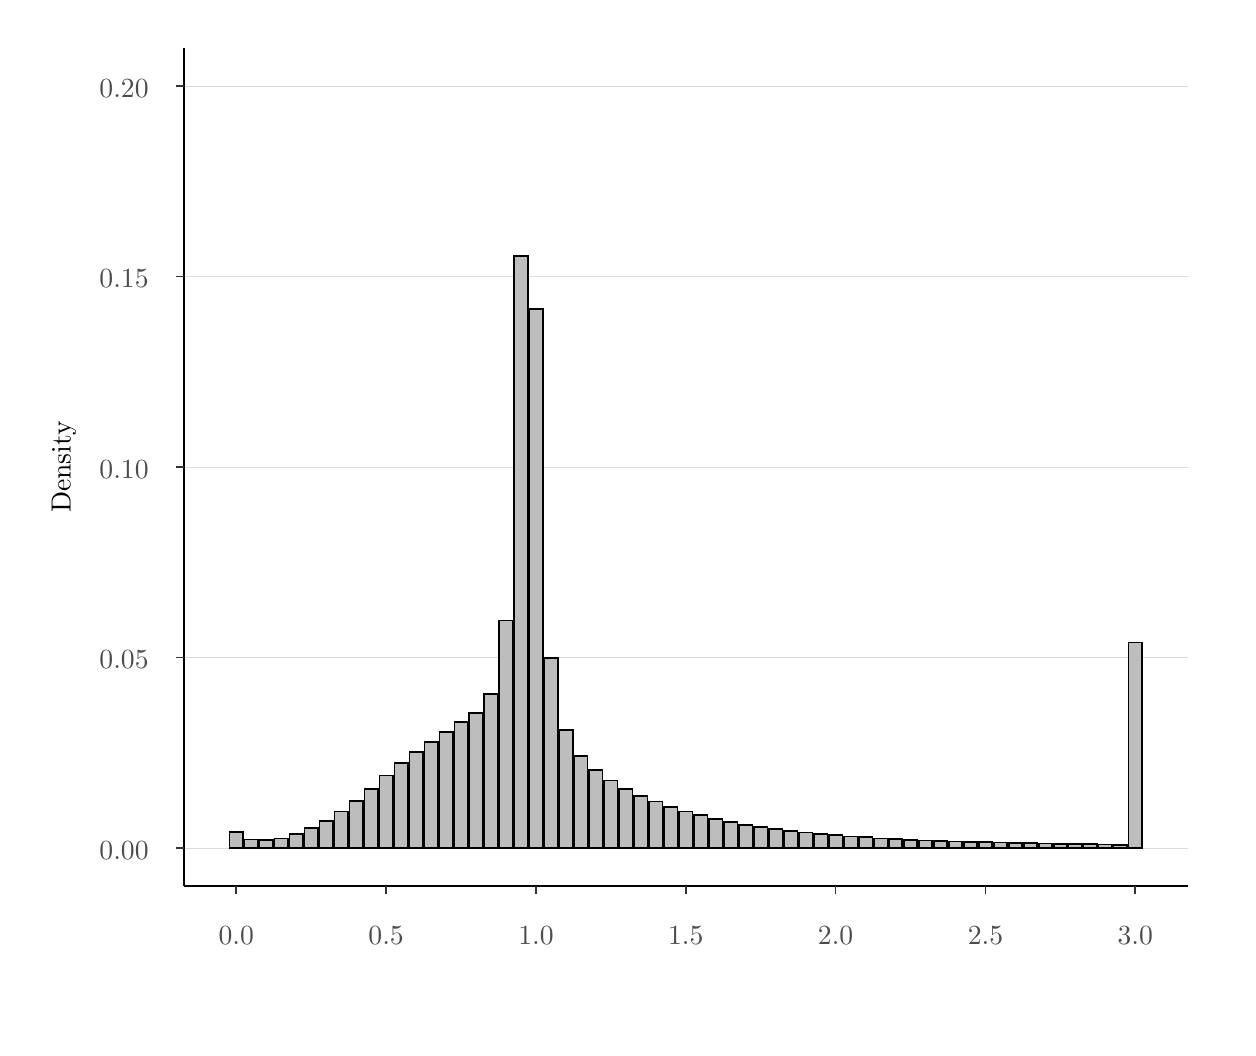
\begin{tikzpicture}[x=1pt,y=1pt]
\definecolor{fillColor}{RGB}{255,255,255}
\path[use as bounding box,fill=fillColor,fill opacity=0.00] (0,0) rectangle (433.62,361.35);
\begin{scope}
\path[clip] (  0.00,  0.00) rectangle (433.62,361.35);
\definecolor{drawColor}{RGB}{255,255,255}
\definecolor{fillColor}{RGB}{255,255,255}

\path[draw=drawColor,line width= 0.6pt,line join=round,line cap=round,fill=fillColor] ( -0.00,  0.00) rectangle (433.62,361.35);
\end{scope}
\begin{scope}
\path[clip] ( 56.47, 51.15) rectangle (419.17,354.12);
\definecolor{drawColor}{RGB}{255,255,255}

\path[draw=drawColor,line width= 0.3pt,line join=round] ( 56.47, 99.35) --
	(419.17, 99.35);

\path[draw=drawColor,line width= 0.3pt,line join=round] ( 56.47,168.21) --
	(419.17,168.21);

\path[draw=drawColor,line width= 0.3pt,line join=round] ( 56.47,237.07) --
	(419.17,237.07);

\path[draw=drawColor,line width= 0.3pt,line join=round] ( 56.47,305.92) --
	(419.17,305.92);

\path[draw=drawColor,line width= 0.3pt,line join=round] (102.46, 51.15) --
	(102.46,354.12);

\path[draw=drawColor,line width= 0.3pt,line join=round] (156.60, 51.15) --
	(156.60,354.12);

\path[draw=drawColor,line width= 0.3pt,line join=round] (210.74, 51.15) --
	(210.74,354.12);

\path[draw=drawColor,line width= 0.3pt,line join=round] (264.89, 51.15) --
	(264.89,354.12);

\path[draw=drawColor,line width= 0.3pt,line join=round] (319.03, 51.15) --
	(319.03,354.12);

\path[draw=drawColor,line width= 0.3pt,line join=round] (373.17, 51.15) --
	(373.17,354.12);
\definecolor{drawColor}{gray}{0.85}

\path[draw=drawColor,line width= 0.1pt,line join=round] ( 56.47, 64.92) --
	(419.17, 64.92);

\path[draw=drawColor,line width= 0.1pt,line join=round] ( 56.47,133.78) --
	(419.17,133.78);

\path[draw=drawColor,line width= 0.1pt,line join=round] ( 56.47,202.64) --
	(419.17,202.64);

\path[draw=drawColor,line width= 0.1pt,line join=round] ( 56.47,271.49) --
	(419.17,271.49);

\path[draw=drawColor,line width= 0.1pt,line join=round] ( 56.47,340.35) --
	(419.17,340.35);
\definecolor{drawColor}{RGB}{0,0,0}
\definecolor{fillColor}{gray}{0.74}

\path[draw=drawColor,line width= 0.6pt,line cap=rect,fill=fillColor] ( 72.95, 64.92) rectangle ( 77.82, 70.68);

\path[draw=drawColor,line width= 0.6pt,line cap=rect,fill=fillColor] ( 78.37, 64.92) rectangle ( 83.24, 67.96);

\path[draw=drawColor,line width= 0.6pt,line cap=rect,fill=fillColor] ( 83.78, 64.92) rectangle ( 88.65, 67.82);

\path[draw=drawColor,line width= 0.6pt,line cap=rect,fill=fillColor] ( 89.19, 64.92) rectangle ( 94.07, 68.39);

\path[draw=drawColor,line width= 0.6pt,line cap=rect,fill=fillColor] ( 94.61, 64.92) rectangle ( 99.48, 69.89);

\path[draw=drawColor,line width= 0.6pt,line cap=rect,fill=fillColor] (100.02, 64.92) rectangle (104.90, 72.04);

\path[draw=drawColor,line width= 0.6pt,line cap=rect,fill=fillColor] (105.44, 64.92) rectangle (110.31, 74.73);

\path[draw=drawColor,line width= 0.6pt,line cap=rect,fill=fillColor] (110.85, 64.92) rectangle (115.72, 78.10);

\path[draw=drawColor,line width= 0.6pt,line cap=rect,fill=fillColor] (116.27, 64.92) rectangle (121.14, 81.79);

\path[draw=drawColor,line width= 0.6pt,line cap=rect,fill=fillColor] (121.68, 64.92) rectangle (126.55, 86.29);

\path[draw=drawColor,line width= 0.6pt,line cap=rect,fill=fillColor] (127.09, 64.92) rectangle (131.97, 91.12);

\path[draw=drawColor,line width= 0.6pt,line cap=rect,fill=fillColor] (132.51, 64.92) rectangle (137.38, 95.52);

\path[draw=drawColor,line width= 0.6pt,line cap=rect,fill=fillColor] (137.92, 64.92) rectangle (142.80, 99.56);

\path[draw=drawColor,line width= 0.6pt,line cap=rect,fill=fillColor] (143.34, 64.92) rectangle (148.21,103.34);

\path[draw=drawColor,line width= 0.6pt,line cap=rect,fill=fillColor] (148.75, 64.92) rectangle (153.62,106.76);

\path[draw=drawColor,line width= 0.6pt,line cap=rect,fill=fillColor] (154.17, 64.92) rectangle (159.04,110.44);

\path[draw=drawColor,line width= 0.6pt,line cap=rect,fill=fillColor] (159.58, 64.92) rectangle (164.45,113.75);

\path[draw=drawColor,line width= 0.6pt,line cap=rect,fill=fillColor] (164.99, 64.92) rectangle (169.87,120.67);

\path[draw=drawColor,line width= 0.6pt,line cap=rect,fill=fillColor] (170.41, 64.92) rectangle (175.28,147.18);

\path[draw=drawColor,line width= 0.6pt,line cap=rect,fill=fillColor] (175.82, 64.92) rectangle (180.70,278.85);

\path[draw=drawColor,line width= 0.6pt,line cap=rect,fill=fillColor] (181.24, 64.92) rectangle (186.11,259.61);

\path[draw=drawColor,line width= 0.6pt,line cap=rect,fill=fillColor] (186.65, 64.92) rectangle (191.52,133.47);

\path[draw=drawColor,line width= 0.6pt,line cap=rect,fill=fillColor] (192.07, 64.92) rectangle (196.94,107.53);

\path[draw=drawColor,line width= 0.6pt,line cap=rect,fill=fillColor] (197.48, 64.92) rectangle (202.35, 98.23);

\path[draw=drawColor,line width= 0.6pt,line cap=rect,fill=fillColor] (202.89, 64.92) rectangle (207.77, 93.16);

\path[draw=drawColor,line width= 0.6pt,line cap=rect,fill=fillColor] (208.31, 64.92) rectangle (213.18, 89.35);

\path[draw=drawColor,line width= 0.6pt,line cap=rect,fill=fillColor] (213.72, 64.92) rectangle (218.60, 86.27);

\path[draw=drawColor,line width= 0.6pt,line cap=rect,fill=fillColor] (219.14, 64.92) rectangle (224.01, 83.82);

\path[draw=drawColor,line width= 0.6pt,line cap=rect,fill=fillColor] (224.55, 64.92) rectangle (229.42, 81.72);

\path[draw=drawColor,line width= 0.6pt,line cap=rect,fill=fillColor] (229.97, 64.92) rectangle (234.84, 79.80);

\path[draw=drawColor,line width= 0.6pt,line cap=rect,fill=fillColor] (235.38, 64.92) rectangle (240.25, 78.17);

\path[draw=drawColor,line width= 0.6pt,line cap=rect,fill=fillColor] (240.79, 64.92) rectangle (245.67, 76.75);

\path[draw=drawColor,line width= 0.6pt,line cap=rect,fill=fillColor] (246.21, 64.92) rectangle (251.08, 75.32);

\path[draw=drawColor,line width= 0.6pt,line cap=rect,fill=fillColor] (251.62, 64.92) rectangle (256.50, 74.25);

\path[draw=drawColor,line width= 0.6pt,line cap=rect,fill=fillColor] (257.04, 64.92) rectangle (261.91, 73.33);

\path[draw=drawColor,line width= 0.6pt,line cap=rect,fill=fillColor] (262.45, 64.92) rectangle (267.32, 72.52);

\path[draw=drawColor,line width= 0.6pt,line cap=rect,fill=fillColor] (267.86, 64.92) rectangle (272.74, 71.84);

\path[draw=drawColor,line width= 0.6pt,line cap=rect,fill=fillColor] (273.28, 64.92) rectangle (278.15, 71.14);

\path[draw=drawColor,line width= 0.6pt,line cap=rect,fill=fillColor] (278.69, 64.92) rectangle (283.57, 70.47);

\path[draw=drawColor,line width= 0.6pt,line cap=rect,fill=fillColor] (284.11, 64.92) rectangle (288.98, 69.99);

\path[draw=drawColor,line width= 0.6pt,line cap=rect,fill=fillColor] (289.52, 64.92) rectangle (294.39, 69.64);

\path[draw=drawColor,line width= 0.6pt,line cap=rect,fill=fillColor] (294.94, 64.92) rectangle (299.81, 69.14);

\path[draw=drawColor,line width= 0.6pt,line cap=rect,fill=fillColor] (300.35, 64.92) rectangle (305.22, 68.83);

\path[draw=drawColor,line width= 0.6pt,line cap=rect,fill=fillColor] (305.76, 64.92) rectangle (310.64, 68.38);

\path[draw=drawColor,line width= 0.6pt,line cap=rect,fill=fillColor] (311.18, 64.92) rectangle (316.05, 68.15);

\path[draw=drawColor,line width= 0.6pt,line cap=rect,fill=fillColor] (316.59, 64.92) rectangle (321.47, 67.93);

\path[draw=drawColor,line width= 0.6pt,line cap=rect,fill=fillColor] (322.01, 64.92) rectangle (326.88, 67.69);

\path[draw=drawColor,line width= 0.6pt,line cap=rect,fill=fillColor] (327.42, 64.92) rectangle (332.29, 67.48);

\path[draw=drawColor,line width= 0.6pt,line cap=rect,fill=fillColor] (332.84, 64.92) rectangle (337.71, 67.30);

\path[draw=drawColor,line width= 0.6pt,line cap=rect,fill=fillColor] (338.25, 64.92) rectangle (343.12, 67.08);

\path[draw=drawColor,line width= 0.6pt,line cap=rect,fill=fillColor] (343.66, 64.92) rectangle (348.54, 67.04);

\path[draw=drawColor,line width= 0.6pt,line cap=rect,fill=fillColor] (349.08, 64.92) rectangle (353.95, 66.87);

\path[draw=drawColor,line width= 0.6pt,line cap=rect,fill=fillColor] (354.49, 64.92) rectangle (359.37, 66.68);

\path[draw=drawColor,line width= 0.6pt,line cap=rect,fill=fillColor] (359.91, 64.92) rectangle (364.78, 66.64);

\path[draw=drawColor,line width= 0.6pt,line cap=rect,fill=fillColor] (365.32, 64.92) rectangle (370.19, 66.52);

\path[draw=drawColor,line width= 0.6pt,line cap=rect,fill=fillColor] (370.74, 64.92) rectangle (375.61, 66.45);

\path[draw=drawColor,line width= 0.6pt,line cap=rect,fill=fillColor] (376.15, 64.92) rectangle (381.02, 66.34);

\path[draw=drawColor,line width= 0.6pt,line cap=rect,fill=fillColor] (381.56, 64.92) rectangle (386.44, 66.25);

\path[draw=drawColor,line width= 0.6pt,line cap=rect,fill=fillColor] (386.98, 64.92) rectangle (391.85, 66.22);

\path[draw=drawColor,line width= 0.6pt,line cap=rect,fill=fillColor] (392.39, 64.92) rectangle (397.27, 66.07);

\path[draw=drawColor,line width= 0.6pt,line cap=rect,fill=fillColor] (397.81, 64.92) rectangle (402.68,139.23);
\end{scope}
\begin{scope}
\path[clip] (  0.00,  0.00) rectangle (433.62,361.35);
\definecolor{drawColor}{RGB}{0,0,0}

\path[draw=drawColor,line width= 0.6pt,line join=round] ( 56.47, 51.15) --
	( 56.47,354.12);
\end{scope}
\begin{scope}
\path[clip] (  0.00,  0.00) rectangle (433.62,361.35);
\definecolor{drawColor}{gray}{0.30}

\node[text=drawColor,anchor=base east,inner sep=0pt, outer sep=0pt, scale=  1.00] at ( 43.72, 60.79) {0.00};

\node[text=drawColor,anchor=base east,inner sep=0pt, outer sep=0pt, scale=  1.00] at ( 43.72,129.65) {0.05};

\node[text=drawColor,anchor=base east,inner sep=0pt, outer sep=0pt, scale=  1.00] at ( 43.72,198.51) {0.10};

\node[text=drawColor,anchor=base east,inner sep=0pt, outer sep=0pt, scale=  1.00] at ( 43.72,267.36) {0.15};

\node[text=drawColor,anchor=base east,inner sep=0pt, outer sep=0pt, scale=  1.00] at ( 43.72,336.22) {0.20};
\end{scope}
\begin{scope}
\path[clip] (  0.00,  0.00) rectangle (433.62,361.35);
\definecolor{drawColor}{gray}{0.20}

\path[draw=drawColor,line width= 0.6pt,line join=round] ( 53.72, 64.92) --
	( 56.47, 64.92);

\path[draw=drawColor,line width= 0.6pt,line join=round] ( 53.72,133.78) --
	( 56.47,133.78);

\path[draw=drawColor,line width= 0.6pt,line join=round] ( 53.72,202.64) --
	( 56.47,202.64);

\path[draw=drawColor,line width= 0.6pt,line join=round] ( 53.72,271.49) --
	( 56.47,271.49);

\path[draw=drawColor,line width= 0.6pt,line join=round] ( 53.72,340.35) --
	( 56.47,340.35);
\end{scope}
\begin{scope}
\path[clip] (  0.00,  0.00) rectangle (433.62,361.35);
\definecolor{drawColor}{RGB}{0,0,0}

\path[draw=drawColor,line width= 0.6pt,line join=round] ( 56.47, 51.15) --
	(419.17, 51.15);
\end{scope}
\begin{scope}
\path[clip] (  0.00,  0.00) rectangle (433.62,361.35);
\definecolor{drawColor}{gray}{0.20}

\path[draw=drawColor,line width= 0.6pt,line join=round] ( 75.39, 48.40) --
	( 75.39, 51.15);

\path[draw=drawColor,line width= 0.6pt,line join=round] (129.53, 48.40) --
	(129.53, 51.15);

\path[draw=drawColor,line width= 0.6pt,line join=round] (183.67, 48.40) --
	(183.67, 51.15);

\path[draw=drawColor,line width= 0.6pt,line join=round] (237.82, 48.40) --
	(237.82, 51.15);

\path[draw=drawColor,line width= 0.6pt,line join=round] (291.96, 48.40) --
	(291.96, 51.15);

\path[draw=drawColor,line width= 0.6pt,line join=round] (346.10, 48.40) --
	(346.10, 51.15);

\path[draw=drawColor,line width= 0.6pt,line join=round] (400.24, 48.40) --
	(400.24, 51.15);
\end{scope}
\begin{scope}
\path[clip] (  0.00,  0.00) rectangle (433.62,361.35);
\definecolor{drawColor}{gray}{0.30}

\node[text=drawColor,anchor=base,inner sep=0pt, outer sep=0pt, scale=  1.00] at ( 75.39, 30.14) {0.0};

\node[text=drawColor,anchor=base,inner sep=0pt, outer sep=0pt, scale=  1.00] at (129.53, 30.14) {0.5};

\node[text=drawColor,anchor=base,inner sep=0pt, outer sep=0pt, scale=  1.00] at (183.67, 30.14) {1.0};

\node[text=drawColor,anchor=base,inner sep=0pt, outer sep=0pt, scale=  1.00] at (237.82, 30.14) {1.5};

\node[text=drawColor,anchor=base,inner sep=0pt, outer sep=0pt, scale=  1.00] at (291.96, 30.14) {2.0};

\node[text=drawColor,anchor=base,inner sep=0pt, outer sep=0pt, scale=  1.00] at (346.10, 30.14) {2.5};

\node[text=drawColor,anchor=base,inner sep=0pt, outer sep=0pt, scale=  1.00] at (400.24, 30.14) {3.0};
\end{scope}
\begin{scope}
\path[clip] (  0.00,  0.00) rectangle (433.62,361.35);
\definecolor{drawColor}{RGB}{0,0,0}

\node[text=drawColor,rotate= 90.00,anchor=base,inner sep=0pt, outer sep=0pt, scale=  1.00] at ( 15.49,202.64) {Density};
\end{scope}
\end{tikzpicture}
